\shorthandoff{"}
\chapter{Stand der Forschung}
\label{ch:standDerForschung}
\section[Grundlagen]{2.1 Grundlagen}
\label{ch:standDerForschung:grundlagen}
Die im Rahmen dieser Literaturrecherche untersuchten Arbeiten setzen voraus, dass die Fähigkeiten der Mitarbeiter und die für die Stelle benötigten Kompetenzen in einer strukturierten Form vorliegen. Die gängigste Darstellungsart ist dabei eine Matrix, welche über boolsche Werte oder Bewertungen die Ausprägungen der Fähigkeiten jedes Mitarbeiters erfasst \cite[S. 11f.]{recommenderSystems:2016}. Beispiele für Fähigkeits-Matrizen mit boolschen Werten sind in Abbildung \ref{fig:standDerForschung:abb1} dargestellt.\\
\begin{figure}[h]
	\centering
	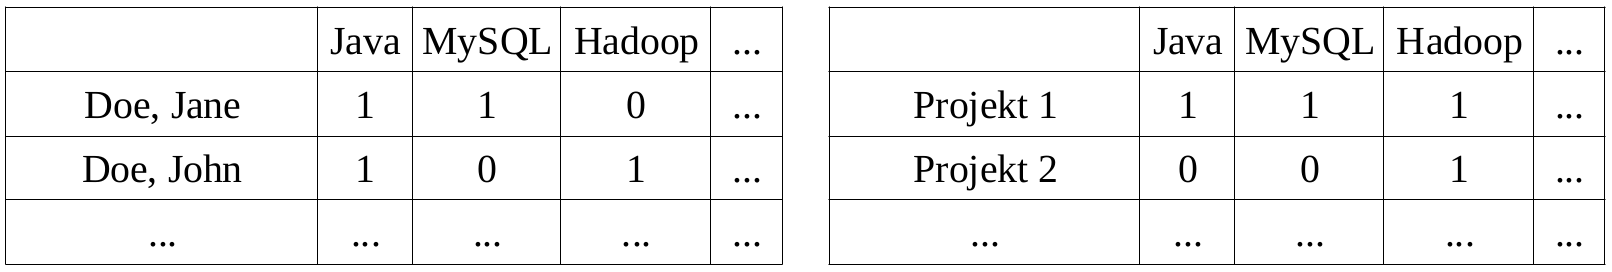
\includegraphics[width=1\textwidth]{gfx/Projektmatrix.png}
	\caption{Beispiele für Matrixdarstellungen von Fähigkeiten}
	\label{fig:standDerForschung:abb1}
\end{figure}
\\
Zahlreiche Wissenschaftler in der Literatur sind sich einig, dass für die Auswahl geeigneter Kandidaten ein einfacher boolscher Abgleich zwischen gesuchten und vorhandenen Fähigkeiten in den Matrizen eine unzureichende Lösung ist \cite[S. 1]{enhancingERecruitment:2012}\cite[S. 1]{faerber:2003}\cite[S. 2]{prospect:2010} und der Komplexität der Aufgabe nicht gerecht wird \cite[S. 1]{malinowski:2008}. So kritisieren beispielsweise \textcite[S. 1f.]{mitre:2014}, dass bei einem solchen Ansatz Synonyme und verwandte Fähigkeit nicht in die Suche einbezogen werden.\\
Aus diesen Gründen ist der gängige Ansatz in der Literatur, ein sogenanntes "Empfehlungssystem" zu implementieren. Im englischsprachigen Raum ist dieser Begriff unter der Bezeichnung "Recommender System" verbreitet und wurde erstmals im Jahr 1997 von \textcite{resnick:1997} geprägt. Ein Empfehlungssystem verfolgt das Ziel, für eine große Menge von Elementen vorherzusagen, wie gut diese für die Anfrage eines Nutzers geeignet sind und sie in der entsprechenden Reihenfolge zu sortieren \cite[S. 3]{recommenderSystems:2016}. Dabei entfällt für den Anwender die Notwendigkeit der manuellen Suche \cite[S. 1]{comibingCareer:2013}. In der Literatur existieren verschiedene Vorschläge, wie Empfehlungssysteme für die vorliegende Problemstellung implementiert werden können. Ein Ansatz ist die Umsetzung eines wissensbasierten Systems.
\newpage
\section[Wissensbasierte Empfehlungssysteme]{2.2 Wissensbasierte Empfehlungssysteme}
\label{ch:standDerForschung:wissensbasierteAnsaetze}
Bei einem wissensbasierten Empfehlungssystem werden die Schlüsselwörter der Matrizen aus Abbildung \ref{fig:standDerForschung:abb1} um weiteres Domänenwissen angereichert, welches in die Suche einbezogen wird \cite[S. 168f.]{recommenderSystems:2016}. So erweitert beispielsweise die Anwendung SAP R/3 Human Resources die Kompetenzen der hinterlegten Kandidaten um eine Fähigkeiten-Ontologie \cite[S. 2]{malinowski:2006}. \textcite[S. 3]{bianchini:2008} stellen bei solch semantischen Ansätzen eine hohe Genauigkeit der Resultate fest, bemängeln jedoch die Flexibilität der Suchverfahren. Obwohl diese Systeme sowohl Synonyme als auch Abhängigkeiten berücksichtigen, werden Mitarbeiter in den Ergebnissen nur ausgegeben, wenn sie die Suchanfrage exakt erfüllen. Aus diesem Grund implementierten \textcite[S. 4ff.]{semanticMatchmaking:2009} ein wissensbasiertes Empfehlungssystem, welches neben einer hohen Genauigkeit zusätzliche Flexibilität gewährleisten sollte. Für dieses Vorhaben entwickelten die Wissenschaftler eine Ontologie, welche die Fähigkeiten der Mitarbeiter sehr feingranular erfasst. Einzelne Kompetenzen müssen dabei über mehrere Einträge spezifiziert werden. Mit diesem Ansatz erreichten \textcite[S. 11f.]{semanticMatchmaking:2009} ihr Ziel, ein genaues und zugleich flexibles wissensbasiertes Empfehlungssystem zu implementieren. Jedoch erscheint die Pflege der Fähigkeiten in der Ontologie derart aufwändig, dass in Frage gestellt werden muss, ob Mitarbeiter ein solches System zuverlässig im Unternehmensalltag pflegen würden. So beobachteten \textcite[S. 2]{aCombinedRepresentation:2018} in anderen, manuell gepflegten Job-Ontologien, dass Informationen über Fähigkeiten häufig nicht aktuell gehalten werden. \\
Sofern die Ergebnisse nicht vollständiger Präzision unterliegen müssen, ziehen Wissenschaftler daher die Entwicklung flexiblerer Empfehlungssysteme den wissensbasierten Ansätzen vor. Meist entstehen dabei Implementierungen im Bereich des kollaborativen oder inhaltsbasierten Filterns.

\section[Kollaboratives und inhaltsbasiertes Filtern]{2.3 Kollaboratives und inhaltsbasiertes Filtern}
\label{ch:standDerForschung:cfundcb}
Empfehlungssysteme im Bereich des kollaborativen oder inhaltsbasierten Filterns nutzen die Daten zusätzlicher Mitarbeiter und Projekte zur Bestimmung von Vorschlägen \cite[S. 8]{recommenderSystems:2016}.\\
Implementierungen auf Basis des kollaborativen Filterns fokussieren die Daten anderer Mitarbeiter. Dabei werden dem Anwender Stellen empfohlen, für welche sich auch andere Nutzer interessieren, die ihm ähnlich sind \cite[S. 3]{jobMatcher:2020}. Diese Art von Empfehlungssystem ist für die vorliegende Problemstellung jedoch ungeeignet, da hier Mitarbeiter für Projekte empfohlen werden sollen und nicht umgekehrt. Dieses Problem identifizierten auch \textcite[S. 2]{mitre:2014}. Um dennoch ein System auf Basis des kollaborativen Filterns entwickeln zu können, entwarfen die Forscher einen fiktiven "Pseudo-Mitarbeiter". Diesem wiesen sie alle für das Projekt relevanten Fähigkeiten zu. Über Ähnlichkeitsmaße wurden die Angestellten ausgewählt, welche die höchste Übereinstimmung mit dem Pseudo-Mitarbeiter vorweisen konnten. Zu diesem Ansatz muss kritisch angemerkt werden, dass es sich entgegen der Angabe der Wissenschaftler nicht um kollaboratives, sondern um inhaltsbasiertes Filtern handelt.\\
Beim inhaltsbasierten Filtern werden Mitarbeiter für Projekte empfohlen, welche in ihren Fähigkeiten eine möglichst hohe Übereinstimmung mit den im Projekt benötigten Kompetenzen aufweisen \cite[S. 139]{recommenderSystems:2016}. So verwendeten \textcite[S. 2]{mitre:2014} zwar einen Pseudo-Mitarbeiter, dieser stellte jedoch lediglich eine Repräsentation der im Projekt geforderten Fähigkeiten da.\\
Einen ähnlichen Ansatz verfolgten auch \textcite[S. 6ff.]{buildingVectorRepresentations:2020}. Diese stellten die Fähigkeiten der Mitarbeiter und die im Projekt benötigten Kompetenzen in Form von Vektoren dar. Auch hier wurden über Ähnlichkeitsalgorithmen diejenigen Kandidaten ausgewählt, welche die höchste Übereinstimmung mit den gesuchten Fähigkeiten aufweisen konnten.\\
Solche, auf Ähnlichkeitsberechnungen basierende Implementierung, werden als "speicherbasierte Ansätze" bezeichnet. Darüber hinaus existieren auch "modellbasierte Ansätze", welche Verfahren aus dem Bereich des maschinellen Lernens und des Data Minings zur Generierung von Empfehlungen verwenden \cite[S. 9]{recommenderSystems:2016}. So entwickelten beispielsweise \textcite[S. 5ff.]{personJobFit:2018} ein Empfehlungssystem auf Basis eines neuronalen Netzes, welches die Eignung einer Person für eine Stelle aus vergangenen Bewerbungsdaten vorhersagt.\\
Ob eine speicher- oder modellbasierte Implementierung geeigneter ist, muss im Einzelfall entschieden werden. \textcite[S. 4]{peerToPeer:2008} stellen diesbezüglich fest, dass speicherbasierte Ansätze in der Praxis häufig wesentlich einfacher umzusetzen sind, da weniger Parameter aufeinander abgestimmt werden müssen. Modellbasierte Ansätze benötigen dafür eine kürzere Berechnungszeit, welche laut \textcite[S. 2]{weightedSimilarity:2015} insbesondere bei steigender Datenmenge vorteilhaft ist. Außerdem bieten modellbasierte Verfahren einen einfacheren Umgang mit dem Cold Start- und dem Sparse Data-Problem \cite[S. 4]{peerToPeer:2008}.

\section[Cold Start- und Sparse Data-Problem]{2.4 Cold Start- und Sparse Data-Problem}
\label{ch:standDerForschung:coldStartUndSparseData}
Algorithmen im Bereich des kollaborativen bzw. inhaltsbasierten Filterns setzen voraus, dass ausreichend Fähigkeits-Daten der Mitarbeiter vorhanden sind. Verfügt ein Angestellter ausschließlich über Fähigkeiten, welche kein anderer Mitarbeiter besitzt oder welche für kein Projekt exklusiv ausgeschrieben sind, wird dieser von den bisher vorgestellten Verfahren im Empfehlungsprozess nicht berücksichtigt. Dieses Phänomen wird als "Cold Start"-Problem bezeichnet \cite[S. 1]{coldStart:2002}. Um ihm entgegenzuwirken, ist in der Literatur die Implementierung hybrider Verfahren verbreitet. Diese kombinieren Ansätze des kollaborativen und inhaltsbasierten Filterns innerhalb eines Systems \cite[S. 8]{malinowski:2008}. So konnten beispielsweise \textcite[S. 8]{combiningCbAndCFCostSensitiveApproach:2017} nachweisen, dass sie durch die Implementierung eines hybriden Verfahrens die Empfehlungen bei Stellensuchen verbessern konnten. \textcite[S. 16]{hybridImmunizing:2017} zeigten, dass deren hybrides Job-Empfehlungssystem trotz der Kombination von kollaborativem und inhaltsbasiertem Filtern eine nach wie vor sehr hohe Performance aufweisen konnte.\\
Neben dem Cold Start sollten Empfehlungssysteme auch eine Lösung für das Sparse Data-Problem bieten. Dieses bezeichnet das Phänomen, dass in der Praxis für einen Großteil der Fähigkeiten nur sehr wenige Bewertungen vorliegen \cite[S. 8]{recommenderSystems:2016}. So stellten \textcite[S. 3]{mitre:2014} bei der Implementierung ihres Projekt-Empfehlungssystems fest, dass über die Hälfte der ca. 17.000 vergebenen Fähigkeiten von nur je einem Mitarbeiter angegeben wurden. Um auch bei einer solch geringen Datendichte Empfehlungen generieren zu können, schlagen einige Wissenschaftler auch hier die Implementierung hybrider Verfahren vor \cite[S. 3]{weightedSimilarity:2015}.\\
\textcite[S. 1]{malinowski:2008} kritisieren jedoch, dass auch ein hybrides Empfehlungssystem nicht ausreicht, um Mitarbeiter für Projekte zu empfehlen. Deren Einschätzung zu Folge ist die Implementierung eines bilateralen Empfehlungssystems notwendig.

\section[Bilaterale Empfehlungssysteme]{2.5 Bilaterale Empfehlungssysteme}
\label{ch:standDerForschung:bilateraleVerfahren}
Die Idee des bilateralen Empfehlungssystems basiert auf der Arbeit von Jeffrey R. Edwards, einem Forscher im Bereich des organisationalen Verhaltens \cite[S. 3]{malinowski:2006}. \textcite[S. 2ff.]{edwards:1991} untersuchte, unter welchen Bedingungen eine Person grundsätzlich für eine Stelle geeignet ist. Dabei stellte er fest, dass neben der Befähigung des Mitarbeiters für eine bestimmte Position auch dessen Wünsche bzw. Bedürfnisse zur vorgesehenen Stelle passen müssen. Diese zweite Ebene muss laut \textcite[S. 1]{malinowski:2006} ebenfalls von Empfehlungssystemen berücksichtigt werden. Betrachtet ein solches System neben den Anforderungen des Personalsachbearbeiters an die Fähigkeiten des Mitarbeiters auch die Wünsche des Angestellten, sprechen die Wissenschaftler von einem bilateralen Empfehlungssystem.\\
Es ist festzustellen, dass der Wunsch des Mitarbeiters in der Literatur nicht einheitlich interpretiert wird. So entwickelten \textcite[S. 1ff.]{applyingDataMining:2014} ein bilaterales Empfehlungssystem auf Basis von Data Mining-Technologien. Die Wissenschaftler verstehen dabei unter dem Wunsch des Nutzers dessen Präferenz für ein bestimmtes Gehalt oder die Bekanntheit eines potenziellen Arbeitgebers. \textcite[S. 4ff.]{malinowski:2006} interpretieren den Wunsch des Nutzers dagegen als dessen Präferenz für bestimmte Stellenprofile.\\
Allgemein ist festzustellen, dass zu bilateralen Empfehlungssystemen bislang nur sehr wenig Literatur existiert \cite[S. 2f.]{jobRecommenderSystemsASurvey:2012}.\\

% bemerken, dass zu diesem Forschungsgebiet bislang sehr wenig Literatur existiert.\\
%- \cite{applyingDataMining:2014}: Nutzerprofil --> Data Mining --> Klassifikation in Gruppe --> CB unter Einbezug der persönlichen Präferenzen (Präferenzen kommen aus Eingabeformular und werden aus Bewerbungshistorie gemint) / Präferenzen: z.B. lieber besser angesehenes Unternehmen oder mehr Geld / Mehr Fokus auf aktuelle Präferenzen, als Historie / Erstellen Entscheidungsbaum / Beziehen Domänenwissen mit ein, um Skills besser matchen zu können / Fazit: Präferenzen mit einzubeziehen erhöht wie akkurat das Ergebnis ist / Wenn Kandidat einen Karriereweg verfolgt, fokussiert das System auf die letzten Jobs\\
%- \cite{malinowski:2008}: "Existing systems only consider whether a person has the requiredtechnical skills and abilities for a job." / Quelle 2: Existing approaches usually consider only unary attri-butes that are tied directly to an individual (e.g.educational data) and–based on them–assess theaptitude of a candidate in relation to the job requirements\\
%- \cite{jobRecommenderSystemsASurvey:2012}: Quelle 15: Bilaterales Sytstem / Quelle: Piazzato baut Reciporal Reommender für Jobs / Zu Reciprocal wenig Literatur
%- \cite{hybridImmunizing:2017}: Entwickeln hybrides System unter Beachtung des bilateralen Systems \\
%- \cite{malinowski:2006}: Theorie zeigt, dass für ein gutes Match eine bilaterale Beziehung bestehen muss\\
%- \cite{malinowski:2008} orientiert sich an Edwards \cite{edwards:1991}, der sagt, dass man noch die Wunsch-Ebene mit einbeziehen muss / Traditioneller Ansatz in Literatur: Nur Skill-Abgleich --> eigentlich muss man beide Perspektiven mit einbeziehen / Setzt Fokus auf Person-Team Fit / Aktuelle Systeme fokussieren nur auf die Abilities-Ebene --> Auch Match zwischen Person und Team wird nicht berücksichtigt / Quelle 44 und 47 entwickelten RS, die Needs-Supplies beachten \\
%- \cite{comibingCareer:2013}: Vorteil Keyword-Abgleich: Nutzer hat viel Kontrolle --> Kann aber nicht bewerten, ob er auch zu den geeignetsten Kandidaten für den Job gehört / System soll entwickelt werden, bei welchem Nutzern nur Jobs empfohlen werden, welche für ihre Karriere förderlich sind --> Es werden Jobs aus der Historie anderer Nutzer ermittelt / Malinowski: Bilaterale Beziehung --> Benötigt: Reciporal RS --> Vergleich Online-Dating: Dort oft CF, hier aber ungeeignet wegen der Data Sparsity / Nutzen Daten von 2.410 LinkedIn-Nutzern, entfernten aktuellsten Job und versuchten diesen vorauszusagen / Es wird eine Flag eingeführt, welche einen Vertrauenswert in das Ergebnis mit angibt (kann stark oder schwach sein) / Apache OpenNLP überführt Text in Keyworte, wobei ähnliche Begriffe erkannt werden / Baseline: Kosinus-Ähnlichkeit / Entwickeln ein kaskadierenes System, wobei jedes System unabhängig voneinander Empfehlungen macht und diese dann unter Beachtung der Flag von einem Multiplexer kombiniert werden --> Kosinus wird nur verwendet, wenn zu wenig Ergebnisse vorliegen / Einzelne Systeme beziehen sich auf unterschiedliche Abschnitte in CV und Ausschreibung \\
%- \cite{malinowski:2006}: Person-Job Fit ist ein Teilgebiet des P-E Fit --> Konzentriert sich aber nur auf den P-J Fit / Edwards \cite{edwards:1991} sagt, dass man auch den Wunsch mit einbeziehen muss / Bilateral --> Deshab werden zwei Systeme parallel entwickelt (CV-RS und Job-RS) --> Bezieht aber Präferenzen der Kandidaten aus Vergangenheitsdaten mit ein --> Getestet mit Studis \\
%- \cite{edwards:1991}: P-J Fit betrachtet zwei Ebenen (rein psychologische Betrachtung) \\
%- \cite{exploringJobRecommentations:2019}: Versucht Kompetenz-Lücken zu finden (Ähnlich Quelle 6 und 9) --> Fokus auf Design nicht auf technischer Umsetzung / Auch Quelle 7 gut \\
%- \cite{dynamicUserProfile:2013}: Quelle 9 (Gauch et al) entwickelten ein dynamisches Nutzerprofil --> Dynamische Veränderung von Interssen und Präferenzen des Nutzers wurden bedacht \\
%- \cite{aCombinedRepresentation:2018}: Gutes Empfehlungssystem schlägt nicht Job vor, der zu Skills passt, sondern schlägt auch Skills vor, die Person erwerben kann, um neue Position zu erhalten / Quelle 8: Skill-GAP, da zu schnell neue Technologien kommen --> Skill-Gap muss eliminiert werden, daher muss erst der Gap bestimmt werden / Ähnlichkeiten zwischen Skills werden bestimmt, um vorzuschlagen, welcher Skill bei Kandidat noch hinzugefügt werden könnte / Skills werden aus Ausschreibungen und Bewerbungen extrahiert --> 2 Graphen: Skill und Skill-Occurence Graphen --> In einem wird nach Ähnlichkeiten gesucht, um Zukunft vorherzusagen / Ziel: Vorhersage des zukünftigen Jobs basierend auf aktuellem Job --> Dafür 20 Mio. Bewerbungen verwendet / Über O*Net wurden Jobs in verschiedene Gruppen kategorisiert / System empfiehlt Jobs und Skills / Nutzen hybriden Ansatz aus CB und CF
\shorthandon{"}